\section*{Ejercicio}
    Asumiendo que la señal de entrada es la mostrada en la figura, diseñar un sistema LTI tal que permita observar el efecto de utilizar un filtro ideal sobre la señal:
     
    \begin{figure}[H]
        \centering
        \begin{tikzpicture}
            \draw[dashed, gray!20](-1,0) grid (4,3.5);
        	\draw[line width = 0.5mm, ->](-1.5,0)--(4.5, 0) node[right]{$t$};
        	\draw[line width = 0.5mm, ->](0,-0.5)--(0,4) node[above]{$x(t)$};
        	\draw[black, line width = 0.3mm](-0.5,0)--(3.5,3) node[right]{$x(t) = \dfrac{1}{4}t +\dfrac{1}{8}$};
        	\draw[black, line width = 0.3mm](3.5,0)--(3.5,3) node[right]{};
            \draw[dashed, line width = 0.2mm](0,3)--(3.5,3) node[right]{};
        	\foreach \x in {-0.5,1.5,3.5}
        	\draw (\x, 1mm)--(\x, -1mm) node [below]{\scriptsize $\x$};
        	\foreach \y in {3}		
        	\draw (1mm, \y)--(-1mm, \y) node [left]{$1$};
        \end{tikzpicture}
    \end{figure}
    
    Dado que la señal de entrada es de tipo diente de sierra con periodo infinito, su respuesta en frecuencia se puede calcular a partir de la Transformada de Fourier. hadflkasdfhasdlfkhasdlfkhsdanflaksdf hadflkasdfhasdlfkhasdlfkhsdanflaksdf  
